\documentclass[10pt,twocolumn,a4paper]{article}

% ---------------------------------------------------------------------------------------------
% Packages
% ---------------------------------------------------------------------------------------------
\usepackage[T1]{fontenc}
\usepackage[utf8]{inputenc}
\usepackage{lmodern}
\usepackage{microtype}
\usepackage[margin=0.8in,columnsep=0.25in]{geometry}
\usepackage{amsmath,amssymb}
\usepackage{booktabs}
\usepackage{multirow}
\usepackage{tabularx}
\usepackage{graphicx}
\usepackage[table]{xcolor}
\usepackage{tikz}
\usetikzlibrary{arrows.meta,positioning,fit,calc,shapes.geometric}
\usepackage{pgfplots}
\pgfplotsset{compat=1.18}
\usepackage[numbers,sort&compress]{natbib}
\usepackage{enumitem}
\usepackage{caption}
\usepackage{subcaption}
\usepackage[hidelinks]{hyperref}
\usepackage{cleveref}

\captionsetup{font=small,labelfont=bf}
\setlist{nosep,leftmargin=*}

\definecolor{cgdet}{HTML}{0C4A6E}
\definecolor{cgdetfill}{HTML}{E0F2FE}
\definecolor{cgllm}{HTML}{4C1D95}
\definecolor{cgllmfill}{HTML}{EDE9FE}
\definecolor{cgok}{HTML}{059669}
\definecolor{cgbad}{HTML}{DC2626}
\definecolor{cgwarn}{HTML}{D97706}
\definecolor{cggrey}{HTML}{6B7280}
\definecolor{bestrow}{HTML}{EAF4EA}

\newcommand{\HeurAcc}{0.400}
\newcommand{\HeurMacroF}{0.145}
\newcommand{\HeurF}{0.095}
\newcommand{\HeurRec}{0.050}
\newcommand{\HeurPrec}{1.000}
\newcommand{\HeurFPR}{0.0}
\newcommand{\HeurCFPR}{0.0}
\newcommand{\HeurECE}{0.589}
\newcommand{\HeurTok}{0}
\newcommand{\HeurLatP}{0.0}
\newcommand{\HeurLatQ}{0}
\newcommand{\DoiAcc}{0.400}
\newcommand{\DoiMacroF}{0.150}
\newcommand{\DoiF}{0.000}
\newcommand{\DoiRec}{0.000}
\newcommand{\DoiPrec}{0.000}
\newcommand{\DoiFPR}{11.1}
\newcommand{\DoiCFPR}{0.0}
\newcommand{\DoiECE}{0.305}
\newcommand{\DoiTok}{0}
\newcommand{\DoiLatP}{0.0}
\newcommand{\DoiLatQ}{0}
\newcommand{\LlmTwentyAcc}{0.473}
\newcommand{\LlmTwentyMacroF}{0.323}
\newcommand{\LlmTwentyF}{0.706}
\newcommand{\LlmTwentyRec}{0.800}
\newcommand{\LlmTwentyPrec}{0.632}
\newcommand{\LlmTwentyFPR}{31.1}
\newcommand{\LlmTwentyCFPR}{10.0}
\newcommand{\LlmTwentyECE}{0.328}
\newcommand{\LlmTwentyTok}{784}
\newcommand{\LlmTwentyLatP}{6.8}
\newcommand{\LlmTwentyLatQ}{9}
\newcommand{\LlmQwenAcc}{0.367}
\newcommand{\LlmQwenMacroF}{0.264}
\newcommand{\LlmQwenF}{0.587}
\newcommand{\LlmQwenRec}{0.700}
\newcommand{\LlmQwenPrec}{0.506}
\newcommand{\LlmQwenFPR}{45.6}
\newcommand{\LlmQwenCFPR}{31.7}
\newcommand{\LlmQwenECE}{0.294}
\newcommand{\LlmQwenTok}{220}
\newcommand{\LlmQwenLatP}{8.4}
\newcommand{\LlmQwenLatQ}{19}
\newcommand{\LlmBigAcc}{0.327}
\newcommand{\LlmBigMacroF}{0.244}
\newcommand{\LlmBigF}{0.727}
\newcommand{\LlmBigRec}{0.800}
\newcommand{\LlmBigPrec}{0.667}
\newcommand{\LlmBigFPR}{26.7}
\newcommand{\LlmBigCFPR}{13.3}
\newcommand{\LlmBigECE}{0.386}
\newcommand{\LlmBigTok}{671}
\newcommand{\LlmBigLatP}{6.6}
\newcommand{\LlmBigLatQ}{8}
\newcommand{\ExactAcc}{0.967}
\newcommand{\ExactMacroF}{0.970}
\newcommand{\ExactF}{1.000}
\newcommand{\ExactRec}{1.000}
\newcommand{\ExactPrec}{1.000}
\newcommand{\ExactFPR}{0.0}
\newcommand{\ExactCFPR}{0.0}
\newcommand{\ExactECE}{0.015}
\newcommand{\ExactTok}{0}
\newcommand{\ExactLatP}{7.3}
\newcommand{\ExactLatQ}{20}
\newcommand{\NoLlmAcc}{0.960}
\newcommand{\NoLlmMacroF}{0.964}
\newcommand{\NoLlmF}{1.000}
\newcommand{\NoLlmRec}{1.000}
\newcommand{\NoLlmPrec}{1.000}
\newcommand{\NoLlmFPR}{0.0}
\newcommand{\NoLlmCFPR}{0.0}
\newcommand{\NoLlmECE}{0.013}
\newcommand{\NoLlmTok}{0}
\newcommand{\NoLlmLatP}{0.0}
\newcommand{\NoLlmLatQ}{5}
\newcommand{\FullAcc}{0.960}
\newcommand{\FullMacroF}{0.964}
\newcommand{\FullF}{1.000}
\newcommand{\FullRec}{1.000}
\newcommand{\FullPrec}{1.000}
\newcommand{\FullFPR}{0.0}
\newcommand{\FullCFPR}{0.0}
\newcommand{\FullECE}{0.017}
\newcommand{\FullTok}{241}
\newcommand{\FullLatP}{0.0}
\newcommand{\FullLatQ}{52}


\newcommand{\verdict}[1]{\textsc{\MakeLowercase{#1}}}
\newcommand{\cg}{CiteGuard}
\newcommand{\code}[1]{\texttt{\small #1}}
\makeatletter
\newcommand{\tabinput}[1]{\@@input #1 }  % \input that works inside tabular
\makeatother

\title{\textbf{CiteGuard: Evidence-First Detection, Verification\\ and Explanation of Fabricated Citations with LLMs}}
\author{Miten Gandhi\\
\small Introduction to Large Language Models (ILLM) --- Final Project\\
\small \url{https://github.com/mjgandhi2305/ILLM_FinalProject_Citeguard}}
\date{November 2026}

\begin{document}
\maketitle

% =============================================================================================
\begin{abstract}
Large language models (LLMs) now help write scientific text, and they invent references that look
real: plausible titles, real-sounding authors, real venues, even real DOIs that belong to other
papers. Detecting such citations sounds like a natural job for an LLM, but an LLM judging a citation
from memory is itself prone to hallucination and, as we show, wrongly rejects correct citations it
does not recognise. We present \cg{}, a citation verifier built on an \emph{evidence-first}
principle: whether a cited work exists is decided only by retrieval from scholarly indexes
(doi.org, Crossref, OpenAlex, Semantic Scholar, arXiv, PubMed) and deterministic record linkage,
while the LLM is confined to tasks that evidence can check: parsing messy references,
choosing among retrieved candidates, rewriting failed searches, writing explanations whose every
claim must cite evidence, and an opt-in check of whether the cited abstract supports the citing
sentence. \cg{} assigns one of five verdicts (verified, verified with errors, misattributed,
fabricated, unverifiable), explains it, and proposes a corrected citation or real alternatives. We
also build CiteBench, a benchmark of real, perturbed and fabricated citations, and evaluate with a
held-out protocol in which every split is scored once before its errors are examined. On a fresh
held-out split of 150 citations, the deterministic pipeline reaches \NoLlmAcc{} five-class accuracy
and \NoLlmF{} fake-detection F1 while calling \NoLlmCFPR\% of correct citations fake. The strongest
LLM-only baseline (\texttt{gpt-oss-120b}) reaches \LlmBigF{} F1 and calls \LlmBigCFPR\% of correct
citations fake, and a DOI-lookup baseline detects none of the fabrications. LLM explanations pass a
grounding validator in 19 of 19 cases, and the claim-support check flags 92\% of mismatched claims
with no false alarms on 25 papers.
\end{abstract}

% =============================================================================================
\section{Introduction}
\label{sec:intro}

Citations are how a paper hands its claims off to evidence. When a writer asks an LLM for
``related work with references'', the model produces citation-shaped strings, and a sizable share of
them do not exist. \citet{walters2023fabrication} found that 55\% of the references produced by
GPT-3.5 and 18\% of those produced by GPT-4 in short literature reviews were fabricated, and that
many real references carried substantive errors; medical-domain studies report similar rates
\citep{bhattacharyya2023high,alkaissi2023artificial,chelli2024hallucination}. These references now
reach the record: an audit of 111 million references in arXiv, bioRxiv, SSRN and PubMed Central
estimates 146,932 non-existent citations in 2025 alone \citep{zhao2026wild}, and hallucinated
references have been found in accepted NeurIPS 2025 papers \citep{kim2026hallmark}. Reviewers cannot
check every reference by hand, so automatic verification has become part of the review process.

The obvious tool is an LLM: ask it whether a reference is real. This fails for a structural reason.
A model that judges a citation from its parametric memory is subject to the same hallucination it is
asked to detect \citep{ji2023survey,huang2025survey}. It recognises famous papers and distrusts
everything else, so it flags most fabrications only because it also flags many obscure real papers.
HALLMARK \citep{kim2026hallmark} measured exactly this on BibTeX entries: zero-shot LLM verifiers
span an order of magnitude in false-positive rate (FPR), from 4\% to 70\%, and giving them database
lookups as tools raised recall but also raised FPR. Because every flag costs a human review, the FPR
on real citations, not recall, decides whether a verifier is usable. Retrieval-only checkers have the
opposite weakness. A DOI resolver cannot see a fabricated title that carries a real DOI, and a
binary found/not-found search conflates ``not indexed'' (books, theses, recent or non-English work)
with ``does not exist'', and gives the user nothing to act on.

Our insight is that existence is a question of \emph{evidence}, not of \emph{judgement}, and that
the LLM is most useful exactly where its output can be checked against that evidence. We build
\cg{} around this division of labour (\cref{fig:pipeline}). Identifiers are extracted by regex and
resolved; the reference is searched in several scholarly indexes; a calibrated record-linkage model
scores each candidate; and deterministic rules map the field-level comparison to a verdict. The LLM
parses references that rules cannot, adjudicates only among retrieved candidates, proposes new
search queries when nothing matches (the code runs them), explains verdicts under a validator that
rejects any claim not present in the evidence, and, on request, judges whether the cited abstract
supports the citing sentence, quoting the abstract verbatim. The LLM never decides that a paper
exists.

We make four contributions:
\begin{itemize}
  \item \textbf{An evidence-first verifier} with a five-verdict taxonomy that separates fabricated
  from misattributed citations and from real citations with errors, and that answers
  \verdict{UNVERIFIABLE} rather than ``fake'' when coverage is thin. Every verdict carries an
  evidence bundle and a validated explanation, plus a corrected citation or real alternatives.
  \item \textbf{A grounded claim-support check} that catches a real paper cited for something it
  does not say, and that discards any judgement whose supporting quote is not verbatim in the
  abstract.
  \item \textbf{CiteBench and a held-out protocol.} Four splits of real, perturbed and fabricated
  citations sampled from two indexes; each split is scored once before its errors are studied.
  \item \textbf{An empirical comparison} against offline heuristics, a DOI-lookup baseline, and three
  LLM-only judges, with an ablation of the pipeline and an error analysis of every failure found.
\end{itemize}
On a fresh held-out split, \cg{} detects every fake citation without a single false alarm on a real
one, while LLM-only judges call 10--32\% of correct citations fake (\cref{sec:results}). The system is released as a web application, a
REST API and a command-line tool.

% =============================================================================================
\section{Related Work}
\label{sec:related}

\paragraph{Measuring citation hallucination.}
Studies of chatbot-written bibliographies report fabrication rates from about one in five to over
half, depending on model and domain
\citep{walters2023fabrication,bhattacharyya2023high,alkaissi2023artificial,chelli2024hallucination}.
Large-scale audits show the problem in published and preprint literature \citep{zhao2026wild} and
in citation URLs produced by deep-research agents \citep{rao2026detecting}. These works measure the
problem; we build a detector and measure its errors, especially false alarms on real citations.

\paragraph{Citation verifiers.}
\citet{agrawal2024hallucinating} detect hallucinated references \emph{without} external resources by
asking the model consistency questions (for example, who the authors are) and observing that models
answer inconsistently about references they invented. This is attractive when no index is
available, but it inherits the model's coverage gaps. Retrieval-based verifiers appeared in
2026. HalluCiteChecker \citep{sakai2026hallucitechecker} is a lightweight offline toolkit; CiteCheck
\citep{khajavi2026citecheck} retrieves candidates from arXiv, Crossref, Semantic Scholar and OpenAlex
and lets an LLM score the citation--candidate pair into exact, minor and major labels; CiteTracer
\citep{li2026source} cascades extraction, retrieval, deterministic field matching and class-specific
LLM judges over a 12-code taxonomy; CiteAudit \citep{shi2026citeaudit} uses a multi-agent pipeline
and a large benchmark; and the AtomGPT checker \citep{neralla2026hallucination} combines LLM field
extraction with Semantic Scholar retrieval. HALLMARK \citep{kim2026hallmark} evaluates such verifiers
under one protocol and argues that FPR limits deployment. \cg{} shares the retrieval-first design of
CiteCheck and CiteTracer but differs in three ways: the verdict is produced by calibrated linkage and
rules rather than an LLM score, so the LLM cannot turn a non-match into a match; explanations are
validated against the evidence before they are shown; and it checks claim support, which CiteCheck
lists as out of scope. Our DOI-lookup baseline follows HALLMARK's.

\paragraph{Hallucination detection and grounded generation.}
General hallucination detectors compare samples for self-consistency \citep{manakul2023selfcheckgpt}
or decompose text into atomic facts checked against a knowledge source \citep{min2023factscore}.
Retrieval-augmented generation grounds outputs in retrieved passages \citep{lewis2020retrieval}, and
\citet{gao2023enabling} evaluate whether generated citations support the generated statements. Our
explanation validator applies the same idea narrowly: every reason must cite an evidence item, and
every quoted value must occur in the evidence.

\paragraph{Claim verification.}
FEVER \citep{thorne2018fever} and SciFact \citep{wadden2020fact} frame verification as labelling a
claim as supported or refuted by retrieved evidence. SemanticCite \citep{haan2025semanticcite}
applies this to citations with full-text retrieval and fine-tuned models. Our claim-support check is
deliberately lighter: abstract-only, opt-in, and presented as a hint, with a verbatim-quote
requirement that makes ungrounded judgements impossible to display.

\paragraph{Reference parsing and record linkage.}
Reference strings are parsed by CRF-based tools such as GROBID \citep{lopez2009grobid}, whose
accuracy depends on style and domain \citep{tkaczyk2018machine}. Matching a parsed reference to an
index record is a record-linkage problem in the sense of \citet{fellegi1969theory}. We rely on open
scholarly metadata from Crossref \citep{hendricks2020crossref}, OpenAlex \citep{priem2022openalex}
and Semantic Scholar \citep{kinney2023semantic}.

% =============================================================================================
\section{Problem Formulation}
\label{sec:problem}

The input is a document, a BibTeX file, a reference list or a single citation, optionally with the
sentences that cite each reference. For each citation $c$, the system outputs a verdict
$v(c)\in\{$\verdict{VERIFIED}, \verdict{VERIFIED\_WITH\_ERRORS}, \verdict{MISATTRIBUTED},
\verdict{FABRICATED}, \verdict{UNVERIFIABLE}$\}$, a confidence, a set of field-level discrepancy codes
with the evidence behind each, an explanation, and a suggestion.
\begin{itemize}
  \item \verdict{VERIFIED}: a real record matches and key fields agree.
  \item \verdict{VERIFIED\_WITH\_ERRORS}: a real record matches, but the year, venue, pages or
  identifier are wrong.
  \item \verdict{MISATTRIBUTED}: the title is real but the authors are substantially wrong, the DOI
  points to another work, or the title and authors come from different works (a chimera).
  \item \verdict{FABRICATED}: no plausible record exists in any healthy source although the citation
  has enough metadata to find one, or its identifier is unregistered and nothing matches.
  \item \verdict{UNVERIFIABLE}: the evidence is insufficient, for example for grey literature, when
  sources are down, or when there is too little metadata.
\end{itemize}

We treat \verdict{FABRICATED} $\cup$ \verdict{MISATTRIBUTED} as the positive (``fake'') class and
report precision, recall and F1. The metric users feel most is the \textbf{false-positive rate on
real citations}: the share of citations of real papers, with or without errors, that the system
calls fake. Because a citation with a wrong year arguably ``does not exist exactly as cited'', we
also report the FPR on \emph{correct} citations only, which no reasonable verifier should flag. We
further report five-class accuracy, macro-F1, the expected calibration error (ECE)
\citep{guo2017calibration} of the confidence, latency, and LLM tokens per citation.

% =============================================================================================
\section{The CiteGuard System}
\label{sec:method}

\begin{figure*}[t]
\centering
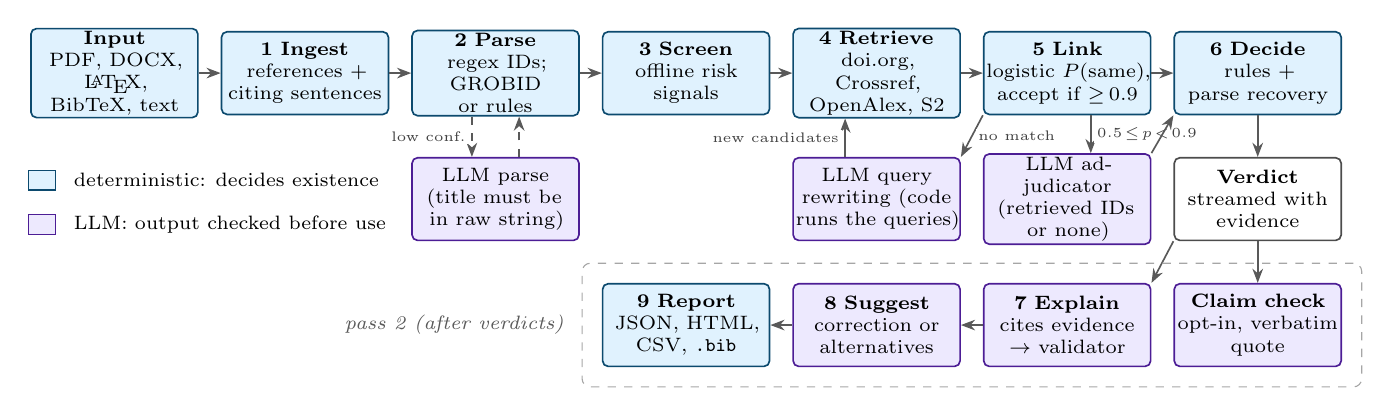
\begin{tikzpicture}[
  x=24.2mm, y=-16mm,
  box/.style={draw=cgdet, fill=cgdetfill, rounded corners=2pt, align=center, font=\scriptsize,
              minimum height=10.5mm, text width=20.5mm, inner sep=1pt, line width=0.6pt},
  llm/.style={box, draw=cgllm, fill=cgllmfill},
  arr/.style={-{Stealth[length=1.8mm]}, line width=0.6pt, draw=black!65},
  lab/.style={font=\tiny, text=black!75, fill=white, inner sep=1pt}
]
% row 1: the deterministic verdict path
\node[box] (in)  at (0,0) {\textbf{Input}\\PDF, DOCX, \LaTeX,\\BibTeX, text};
\node[box] (ing) at (1,0) {\textbf{1 Ingest}\\references +\\citing sentences};
\node[box] (par) at (2,0) {\textbf{2 Parse}\\regex IDs; GROBID\\or rules};
\node[box] (scr) at (3,0) {\textbf{3 Screen}\\offline risk\\signals};
\node[box] (ret) at (4,0) {\textbf{4 Retrieve}\\doi.org, Crossref,\\OpenAlex, S2};
\node[box] (lnk) at (5,0) {\textbf{5 Link}\\logistic $P(\text{same})$,\\accept if ${\ge}\,0.9$};
\node[box] (dec) at (6,0) {\textbf{6 Decide}\\rules +\\parse recovery};
% row 2: LLM helpers, each checked
\node[llm] (lpar) at (2,1) {LLM parse\\(title must be\\in raw string)};
\node[llm] (ref)  at (4,1) {LLM query\\rewriting (code\\runs the queries)};
\node[llm] (adj)  at (5,1) {LLM adjudicator\\(retrieved IDs\\or none)};
\node[box, draw=black!70, fill=white] (ver) at (6,1) {\textbf{Verdict}\\streamed with\\evidence};
% row 3: pass 2
\node[llm] (exp) at (5,2) {\textbf{7 Explain}\\cites evidence\\$\rightarrow$ validator};
\node[llm] (sug) at (4,2) {\textbf{8 Suggest}\\correction or\\alternatives};
\node[box] (rep) at (3,2) {\textbf{9 Report}\\JSON, HTML,\\CSV, \texttt{.bib}};
\node[llm] (clm) at (6,2) {\textbf{Claim check}\\opt-in, verbatim\\quote};

\draw[arr] (in) -- (ing);
\draw[arr] (ing) -- (par);
\draw[arr] (par) -- (scr);
\draw[arr] (scr) -- (ret);
\draw[arr] (ret) -- (lnk);
\draw[arr] (lnk) -- (dec);
\draw[arr, dashed] ([xshift=-3mm]par.south) -- node[lab, left=1pt] {low conf.} ([xshift=-3mm]lpar.north);
\draw[arr, dashed] ([xshift=3mm]lpar.north) -- ([xshift=3mm]par.south);
\draw[arr] (lnk.south west) -- node[lab, pos=0.5, right=1pt] {no match} (ref.north east);
\draw[arr] ([xshift=-4mm]ref.north) -- node[lab, left=1pt] {new candidates} ([xshift=-4mm]ret.south);
\draw[arr] ([xshift=3mm]lnk.south) -- node[lab, right=1pt] {$0.5\!\le\! p\!<\!0.9$} ([xshift=3mm]adj.north);
\draw[arr] (adj.north east) -- (dec.south west);
\draw[arr] (dec) -- (ver);
\draw[arr] (ver.south west) -- (exp.north east);
\draw[arr] (ver) -- (clm);
\draw[arr] (exp) -- (sug);
\draw[arr] (sug) -- (rep);

\node[draw=black!35, dashed, rounded corners=3pt, inner sep=2.5mm, fit=(rep)(sug)(exp)(clm)] (p2) {};
\node[font=\scriptsize\itshape, text=black!65, anchor=east] at ($(p2.west)+(-1mm,0)$) {pass 2 (after verdicts)};

\node[draw=cgdet, fill=cgdetfill, minimum width=3.5mm, minimum height=2.5mm, inner sep=0pt]
  (k1) at (-0.38,0.85) {};
\node[font=\scriptsize, anchor=west] at ($(k1.east)+(1mm,0)$) {deterministic: decides existence};
\node[draw=cgllm, fill=cgllmfill, minimum width=3.5mm, minimum height=2.5mm, inner sep=0pt]
  (k2) at (-0.38,1.2) {};
\node[font=\scriptsize, anchor=west] at ($(k2.east)+(1mm,0)$) {LLM: output checked before use};
\end{tikzpicture}
\caption{\textbf{\cg{} pipeline.} Existence is decided only by blue, deterministic stages
(retrieval, record linkage, rules). Purple stages use the LLM (Groq) for tasks whose output is
checked: the parser's title must occur in the raw string, the adjudicator may only pick a retrieved
candidate, reformulated queries are executed by code and re-scored, explanations must cite evidence
IDs, and claim judgements must quote the abstract verbatim. Verdicts stream to the user after stage
6; explanations, suggestions and claim checks fill in during a second pass.}
\label{fig:pipeline}
\end{figure*}

\Cref{fig:pipeline} shows the pipeline. We describe each stage with its motivation and the design
choice that keeps the LLM from deciding existence.

\subsection{Ingestion, parsing and screening}
\textbf{Ingestion} accepts PDF (through GROBID \citep{lopez2009grobid} when available, otherwise
text extraction and reference-section segmentation), DOCX, \LaTeX{} with \texttt{.bib}, BibTeX,
plain text and single citations. In-text markers such as ``[3]'' or ``(Smith, 2020)'' are linked back
to their references so that the citing sentence travels with the citation.

\textbf{Parsing} extracts DOIs, arXiv IDs, PMIDs and ISBNs by regular expression first; these
identifiers are authoritative and no later step may change them. Fields are then parsed by GROBID,
by a Unicode-aware heuristic parser for APA, IEEE, Vancouver and BibTeX, or, for references whose
parse confidence is low, by the LLM. The LLM parser must transcribe faithfully and its title must
occur (fuzzily) in the raw string; otherwise the next strategy is used.

\textbf{Screening} computes instant offline risk signals (an invalid DOI checksum or prefix, an
arXiv ID whose date disagrees with the year, future dates, impossible pages, an unknown venue). These
are shown immediately and feed the final confidence, but they never decide a verdict alone.

\subsection{Retrieval and record linkage}
\textbf{Retrieval} resolves identifiers at doi.org (which covers every registration agency) and
arXiv, then searches Crossref, OpenAlex and Semantic Scholar, adding PubMed and arXiv by detected
field. Each source sits behind a token-bucket rate limiter, retries with back-off, a circuit
breaker, a cache (30 days for hits, 24 hours for misses) and a hard 20-second deadline per call. A
slow source therefore lowers confidence instead of stalling the job.

\textbf{Linkage} normalises titles and names (NFKC, case and diacritic folding, \LaTeX{}
de-escaping; native-script and transliterated names; particles such as ``van'' and ``dos'') and
computes field features: title similarity, first-author match, author-set precision and F1, year
difference, venue similarity through an alias table, volume, issue and page agreement, and
identifier agreement. A logistic model maps these features to $P(\text{same work})$. Candidates with
$p\ge0.9$ are accepted, those with $p<0.5$ rejected, and the ambiguous band goes to the LLM
adjudicator, which sees the citation and the top three candidates and may answer only with one of
their IDs or ``none''; a similarity floor rejects implausible picks. A chimera check searches by
author and year to detect a real title paired with the authors of a different work.

\textbf{Query reformulation} runs only when nothing matches, and always before a
\verdict{FABRICATED} verdict. The LLM proposes up to four alternative queries (without a subtitle,
with transliterated names, author plus topic); the code runs them for at most two rounds, and the
linkage model scores whatever they return. The LLM therefore only \emph{surfaces candidates}.

\subsection{Decision rules and parse recovery}
Deterministic rules turn the evidence into a verdict. An unregistered DOI yields
\code{ID\_NOT\_REGISTERED} and a search by metadata; a registered DOI whose title differs yields
\code{ID\_RESOLVES\_TO\_DIFFERENT\_WORK}; a matched title whose listed authors are mostly absent from
the record (author precision below 0.5) yields \verdict{MISATTRIBUTED}; and no match in at least two
healthy relevant sources, for an article-like citation with enough metadata, yields
\verdict{FABRICATED}, otherwise \verdict{UNVERIFIABLE}. Author checks use precision rather than F1, so
a correct but truncated author list is a note (\code{AUTHORS\_MISSING}), not a misattribution. The
confidence of a \verdict{FABRICATED} verdict is $1-P(\text{real work missed})$, using retrieval
recall measured on the benchmark.

\textbf{Parse recovery} is a safety net for every parser. Before calling an unconfirmed citation
fabricated, the verifier checks whether some retrieved record's title and first author occur
verbatim in the raw string, as a whole segment between punctuation. If so, the parse was wrong: the
reference is re-parsed around that title and verified again. The segment requirement stops a
hallucination that \emph{extends} a real title (``Attention Is All You Need for protein structure
prediction'') from being rescued.

\subsection{Grounded LLM outputs}
\textbf{Explanations.} Every verdict first receives a deterministic template explanation, so users
see a reason immediately. In a second pass the LLM receives an evidence bundle (claimed fields, each
source response with its status and URL, the best match, field differences, discrepancy codes) in
which every item has an ID, and returns strict JSON with a headline, reasons that cite evidence IDs,
and a recommendation. A validator checks that each cited ID exists, that each quoted title, DOI,
name or number occurs in the bundle, and that the headline does not call a citation fake unless the
verdict is \verdict{FABRICATED} or \verdict{MISATTRIBUTED}. On failure the model gets one retry with
feedback; after that the template explanation stays.

\textbf{Suggestions.} For real citations with errors, the matched record is formatted in the user's
style with a field-level diff and a corrected BibTeX entry. For fabricated citations, candidates are
retrieved by topic (and by the citing sentence when available) from Semantic Scholar and OpenAlex,
and the LLM reranks them by abstract, returning up to three with a relevance note, or none if none
fits.

\textbf{Claim-support check (opt-in).} For a verified citation with a citing sentence, \cg{} fetches
the abstract (from the retrieved records, then by DOI from OpenAlex or Semantic Scholar) and asks the
LLM to label the sentence \textsc{supports}, \textsc{partial}, \textsc{not\_supported} or
\textsc{cannot\_determine}, quoting the abstract. A judgement whose quote does not occur verbatim (after
case and whitespace folding) is retried once and otherwise downgraded to \textsc{cannot\_determine}.
No LLM call is made when no abstract of at least 30 words exists. A \textsc{not\_supported} result
adds the flag \code{CLAIM\_NOT\_SUPPORTED} and triggers a search for papers that do support the
sentence, excluding the cited one.

\subsection{Implementation}
The backend is Python (FastAPI, asynchronous \texttt{httpx}, Pydantic), with PostgreSQL and Redis
in production and SQLite in development; the frontend is React with TypeScript. A Docker Compose
stack includes optional GROBID. All LLM calls go to Groq with strict JSON-schema outputs:
\texttt{gpt-oss-20b} \citep{openai2025gptoss} parses and reformulates, and \texttt{gpt-oss-120b}
adjudicates, explains, reranks and checks claims. A per-model limiter enforces the free-tier budget
(8K tokens per minute, 200K per day); malformed outputs are retried once on the same model, then
fall back to another model, and finally to deterministic behaviour. A check never fails because of
the LLM, and with no API key the system still runs. The repository contains 110 backend and 7
frontend tests.

% =============================================================================================
\section{Experimental Setup}
\label{sec:setup}

\paragraph{CiteBench.}
Each split has 150 items built by one recipe. \emph{Real} (60): random journal articles from
1990--2024, sampled from both OpenAlex and Crossref so that ground truth does not come from a
single index the system also queries, rendered in APA, IEEE, Vancouver or BibTeX, with the DOI kept
in about half. \emph{Perturbed} (60): year shifted by 2--3 years, venue swapped, or a non-existent DOI
(labelled \verdict{VERIFIED\_WITH\_ERRORS}); authors swapped with another paper's, or another real
paper's DOI (\verdict{MISATTRIBUTED}); and an invented title carrying a real DOI, a typical LLM
hallucination (\verdict{FABRICATED}). \emph{Fabricated} (30): invented but plausible titles with
real-looking authors and real venues (\verdict{FABRICATED}). Labels follow from construction.

\paragraph{Held-out protocol.}
We use four splits with disjoint DOIs: \texttt{dev} (seed 7) for development, and \texttt{test}
(seed 23), \texttt{test2} (seed 41) and \texttt{test3} (seed 59), each scored once before anyone looked
at its errors. After its first score, a split's errors were analysed and fixed, so later scores on it
are optimistic and we do not report them as estimates. \texttt{test3} was built for this paper and
scored once with the final code; it is our main result.

\paragraph{Systems compared.}
\begin{itemize}
  \item \textbf{Offline heuristics}: the screening signals alone, thresholded at 0.3.
  \item \textbf{DOI lookup} (HALLMARK's lower-bound baseline \citep{kim2026hallmark}): a citation
  is flagged only if it has a DOI that doi.org does not resolve; citations without a DOI are not
  flagged.
  \item \textbf{LLM-only}: the model is asked whether the publication ``really exists exactly as
  cited, using only your own knowledge'' and answers yes, no or unsure (mapped to
  \verdict{VERIFIED}, \verdict{FABRICATED}, \verdict{UNVERIFIABLE}), with no retrieval and no fallback
  to another model. We test \texttt{gpt-oss-20b}, \texttt{qwen3.8-27b} and \texttt{gpt-oss-120b}, all
  served by Groq.
  \item \textbf{\cg{}}: retrieval with exact identifier and title matching only; the full
  deterministic pipeline (\texttt{no\_llm}); and the full pipeline with the Groq LLM (\texttt{full}).
\end{itemize}

% =============================================================================================
\section{Results}
\label{sec:results}

\begin{table*}[t]
\centering
\caption{\textbf{Main result: fresh held-out split \texttt{test3}} (150 citations, scored once).
Fake = \verdict{FABRICATED} $\cup$ \verdict{MISATTRIBUTED}. ``FPR correct'' is the share of the 60
correct citations called fake; ``FPR real'' adds the 30 real citations with errors. LLM-only
baselines cannot output \verdict{VERIFIED\_WITH\_ERRORS} or \verdict{MISATTRIBUTED}, which caps their
five-class accuracy; compare them on the binary columns.}
\label{tab:test3}
\small
\setlength{\tabcolsep}{5pt}
\begin{tabular}{@{}lcccccccr@{}}
\toprule
 & \multicolumn{2}{c}{Five-class} & \multicolumn{3}{c}{Fake detection} & \multicolumn{2}{c}{FPR (\%)\,$\downarrow$} & LLM \\
\cmidrule(lr){2-3}\cmidrule(lr){4-6}\cmidrule(lr){7-8}
System & Acc.\,$\uparrow$ & M-F1\,$\uparrow$ & P\,$\uparrow$ & R\,$\uparrow$ & F1\,$\uparrow$ & correct & real & tok./cit. \\
\midrule
\tabinput{generated/test3_table.tex}
\bottomrule
\end{tabular}
\end{table*}

\subsection{Main comparison on the fresh held-out split}
\Cref{tab:test3} answers the central question: does grounding the decision in retrieval beat asking
an LLM? Three findings stand out.

\textbf{Retrieval-grounded verification reaches a far better operating point.} Every \cg{} variant
detects all 60 fake citations (recall \NoLlmRec, precision \NoLlmPrec) without calling a single real
citation fake. No baseline comes close: the best LLM-only judge, \texttt{gpt-oss-120b}, reaches a
fake F1 of \LlmBigF{} but calls \LlmBigCFPR\% of the perfectly correct citations fake (and
\LlmBigFPR\% of all real ones); \texttt{qwen3.8-27b} calls \LlmQwenCFPR\% of correct citations fake.

\textbf{A larger model is not a safer judge.} \texttt{gpt-oss-20b} has a lower false-positive rate on
correct citations (\LlmTwentyCFPR\%) than \texttt{gpt-oss-120b} (\LlmBigCFPR\%); the larger model
mostly answers ``unsure'' (40 of 60 correct citations), which is honest but not useful.
\texttt{qwen3.8-27b} also failed to return valid structured output for 27 of 150 citations even
after a retry; these count as ``unsure''.

\textbf{Identifier checks alone miss fabrication entirely.} The DOI-lookup baseline detects none of
the 60 fakes: CiteBench's invented titles either carry no DOI or borrow a real one, which resolves.
Its only flags are the 10 real papers cited with a non-existent DOI, which are real papers with an
error, so they count as false positives. The offline heuristics flag 2 of 60 fakes.

The LLM changes no verdict on this split (its predictions are identical to \texttt{no\_llm}) at
\FullTok{} tokens per citation. All remaining \cg{} errors are six correct citations labelled
\verdict{VERIFIED\_WITH\_ERRORS}, analysed in \cref{sec:errors}.

\begin{table}[t]
\centering
\caption{\textbf{How the LLM-only judges answered on \texttt{test3}}: counts of ``exists'' /
``fake'' / ``unsure'' per gold group. Every ``fake'' in the first two rows is a false alarm on a real
paper.}
\label{tab:llmonly}
\scriptsize
\setlength{\tabcolsep}{2.6pt}
\begin{tabular}{@{}lccc@{\hspace{6pt}}ccc@{\hspace{6pt}}ccc@{}}
\toprule
 & \multicolumn{3}{c}{\texttt{gpt-oss-20b}} & \multicolumn{3}{c}{\texttt{qwen3.8-27b}} & \multicolumn{3}{c}{\texttt{gpt-oss-120b}} \\
\cmidrule(lr){2-4}\cmidrule(lr){5-7}\cmidrule(l){8-10}
Gold group & ex. & fake & uns. & ex. & fake & uns. & ex. & fake & uns. \\
\midrule
\tabinput{generated/llm_only_breakdown.tex}
\bottomrule
\end{tabular}
\end{table}

\subsection{What the LLM-only judges get wrong}
\Cref{tab:llmonly} breaks the LLM-only answers down by gold group. The judges catch most
fabrications (30--37 of 40), but mainly because they distrust what they do not recognise; the same
distrust makes them call 6--19 of 60 correct citations fake. For real papers cited with a small error
(a year off by two, a swapped venue), they mostly answer ``fake'' (16--22 of 30). Under a prompt that
asks whether a work exists ``exactly as cited'' this answer is defensible, which is why we report the
FPR on correct citations separately; but it shows that a yes/no judge cannot tell a typo from a
fabrication. A user receives no corrected citation, no indication of which field is wrong, and no
evidence to check, which are exactly the outputs \cg{}'s five verdicts and discrepancy codes provide.

\subsection{Earlier held-out estimates}
\begin{table}[t]
\centering
\caption{\textbf{First (held-out) scores of the deterministic pipeline} on each split, each with the
code of its time. Latency is p50 / p95 seconds per citation; \texttt{test3} ran on a source cache
already filled by the exact-matching run, so its latency is not comparable.}
\label{tab:heldout}
\scriptsize
\setlength{\tabcolsep}{2.4pt}
\begin{tabular}{@{}lccccccc@{}}
\toprule
Split & Acc. & M-F1 & P & R & FPR\% & ECE & Lat. (s) \\
\midrule
\tabinput{generated/heldout_table.tex}
\bottomrule
\end{tabular}
\end{table}

\Cref{tab:heldout} lists the first score of every held-out split. The code improved between them:
\texttt{test} exposed Vancouver author lists the parser could not read, \texttt{test2} a handful of
smaller parsing gaps (\cref{sec:errors}), and \texttt{test3} measures the final code. Fake recall was
1.000 on every split. The remaining errors were all on real citations: called fake on \texttt{test}
(5 of 90) and \texttt{test2} (1 of 90), and only given a minor-error verdict on \texttt{test3}. The
false-positive rate fell from 5.6\% to 1.1\% to 0\% as parsing failures were fixed.

\subsection{Ablation}
\begin{table*}[t]
\centering
\caption{\textbf{Ablation ladder on \texttt{dev}} (150 citations; development split, not held out).
Each row adds one component. \texttt{full} and LLM-only were measured before the parse-recovery fix.}
\label{tab:ablation}
\small
\setlength{\tabcolsep}{5pt}
\begin{tabular}{@{}lcccccccr@{}}
\toprule
 & \multicolumn{2}{c}{Five-class} & \multicolumn{3}{c}{Fake detection} & \multicolumn{2}{c}{FPR (\%)\,$\downarrow$} & LLM \\
\cmidrule(lr){2-3}\cmidrule(lr){4-6}\cmidrule(lr){7-8}
System & Acc.\,$\uparrow$ & M-F1\,$\uparrow$ & P\,$\uparrow$ & R\,$\uparrow$ & F1\,$\uparrow$ & correct & real & tok./cit. \\
\midrule
\tabinput{generated/dev_table.tex}
\bottomrule
\end{tabular}
\end{table*}

\Cref{tab:ablation} adds components one at a time on \texttt{dev}. Offline heuristics alone find no
fakes: a fabricated citation with a real venue and a plausible title has no surface defect.
Retrieval is the component that matters. On these tidy synthetic citations exact matching already
solves \texttt{dev}, and fuzzy linkage, the full rules and the LLM change nothing measurable. The
held-out \texttt{test3} split confirms this rather than contradicting it: exact matching scores
\ExactAcc{} accuracy against \NoLlmAcc{} for the full deterministic pipeline (a one-citation
difference), and both detect every fake with no false alarm (\cref{tab:test3}). The improvements
that mattered on the held-out splits were in \emph{parsing} and in the decision rules, which both
rungs share (\cref{sec:errors}). \textbf{We therefore found no benchmark evidence that fuzzy linkage
or the LLM improves verdicts on synthetic citations.} Both are designed for inputs CiteBench does not
contain (typos in titles, transliterated names, references a chatbot half-remembers); measuring them
needs the chatbot-written split described in \cref{sec:discussion}. The LLM's measurable contribution
here is in explanations and claim checks, evaluated next.

\subsection{Explanations and claim support}
\paragraph{Grounded explanations.}
On 30 \texttt{dev} citations run with explanations, all 19 non-verified citations received an LLM
explanation, and all 19 passed the grounding validator (100\%; one retry allowed), at 1,972 tokens
per citation. Verified citations keep the template explanation by design. The validator caught one
real defect during development: for a correctly \verdict{UNVERIFIABLE} citation, the LLM wrote
``Could not verify: citation appears fabricated'', which led to the rule that a headline may call a
citation fake only if the verdict says so.

\paragraph{Claim support.}
For 25 real \texttt{test2} papers with abstracts, \texttt{gpt-oss-120b} judged two claims each: the
paper's own concluding sentence with lead-ins such as ``We show that'' removed (should be supported),
and the concluding sentence of a different, random paper (should not be). All 25 own claims were
labelled \textsc{supports} (0 false alarms), and 23 of 25 foreign claims were labelled
\textsc{not\_supported} (92\%); the other two were vague sentences that received the cautious
\textsc{cannot\_determine}. The grounding check dropped one judgement whose quote was not in the
abstract. A check costs about 1.6K tokens uncached. Synthetic claims measure false alarms and gross
topic mismatches, not subtle misuse such as overgeneralising a finding; that needs a hand-labelled
set.

\paragraph{Self-check on this paper's bibliography.}
We ran \cg{} on the 30 entries of this paper's own reference list (\cref{app:selfcheck}). It
verified 28 and flagged two as \verdict{VERIFIED\_WITH\_ERRORS}; none was called fake. Both flags are
false alarms caused by how indexes record a work: Crossref lists a 2009 proceedings paper under its
series (\emph{Lecture Notes in Computer Science}) rather than its proceedings title, and Semantic
Scholar gives an arXiv record's ``volume'' as \texttt{abs/1706.04599}. Such metadata conventions are
the main source of minor false alarms we observed, and they are harmless by design: a
\verdict{VERIFIED\_WITH\_ERRORS} verdict shows the user both values.

\subsection{Error analysis}
\label{sec:errors}
Every error found on \texttt{dev}, \texttt{test} and \texttt{test2} was traced to a cause and fixed
with a regression test (\cref{tab:errors}). The six \texttt{test3} errors were analysed but left
unfixed, so that \texttt{test3} remains a clean held-out estimate. All six are correct citations
labelled \verdict{VERIFIED\_WITH\_ERRORS}, a minor error that still shows the user the matched record:
a title containing ``II.'' that the sentence splitter cut; an IEEE title containing ``(1998)'' whose
parenthesised year was taken for the publication year (2005); a Japanese record with ALL-CAPS names
and the volume ``2017.23''; and three citations rendered from garbled index metadata (for example the
author ``PG Student, D. o. S. E. C. c. J. H. I.''), where the record itself is the problem.

\begin{table}[t]
\centering
\caption{\textbf{Causes of the errors found by the held-out splits} and the Docker smoke test, and
their fixes. ``Real$\to$fake'' are false alarms.}
\label{tab:errors}
\scriptsize
\setlength{\tabcolsep}{3pt}
\begin{tabularx}{\columnwidth}{@{}lXl@{}}
\toprule
Found on & Cause & Effect \\
\midrule
\texttt{dev} & ALL-CAPS Vancouver titles swallowed the journal & real$\to$unverif. \\
\texttt{dev} & Non-Latin names folded to empty strings; CJK family-name order & real$\to$fake \\
\texttt{dev} & Quoted phrase inside a title taken as an IEEE title & real$\to$unverif. \\
\texttt{test} & Vancouver authors such as ``Van Tinteren H'', ``Helland {\AA}'', Unicode hyphens & real$\to$fake (5) \\
\texttt{test} & APA volume ranges read as pages & minor error \\
\texttt{test2} & ``St.~Petersburg'' split as a sentence end & real$\to$fake \\
\texttt{test2} & Brazilian initials (``BVdS''); partial family names in Crossref & parse failure \\
smoke & Correct but truncated author list judged by F1 & real$\to$misattr. \\
\bottomrule
\end{tabularx}
\end{table}

Two patterns stand out. First, almost every false alarm began as a \emph{parsing} failure: the
remainder of an unreadable author list became the ``title'', nothing matched, and a real paper was
called fabricated with high confidence. Parse recovery (\cref{sec:method}) addresses this class
generally rather than one name at a time. Second, fixes interact: changing author fabrication from
F1 to precision broke two \texttt{dev} items, which the regression runs caught before the change
shipped. Re-running all earlier splits after each fix was essential.

\paragraph{Defects found by the demo.}
Recording the demo exposed two LLM-side issues that no benchmark metric showed. The explainer once
returned the headline ``Real paper with errors:'' with nothing after the label; the validator now
rejects a label-only headline and asks again (with a regression test). In the same explanation, one
reason inferred that the citation ``may have been assembled from mixed sources''. It cited real
evidence IDs and quoted nothing false, so it passed the validator, but the inference was not
warranted. The validator checks values and evidence IDs, not reasoning, which is a limit of
string-level grounding.

\subsection{Cost and latency}
The deterministic pipeline uses no LLM tokens. Its median latency is about one second per uncached
citation; the 95th percentile (about 20 seconds) is set by occasional source time-outs, bounded by the
per-call deadline. On the Groq free tier, verdicts in \texttt{full} mode cost \FullTok{} tokens per
citation on \texttt{test3}, and explanations about 2K; explanation latency (19 s median) is dominated by the
tokens-per-minute limit rather than by the pipeline, and verdicts stream before explanations.

% =============================================================================================
\section{Discussion and Limitations}
\label{sec:discussion}

\paragraph{Why evidence first works.}
The LLM-only judges fail in a predictable direction: they confuse ``I do not recognise this paper''
with ``this paper does not exist''. Retrieval reverses the burden of proof: a real paper is found
regardless of how obscure it is, and a fabricated one is not found regardless of how plausible it
sounds. Separating \verdict{FABRICATED} from \verdict{UNVERIFIABLE} keeps thin coverage from turning
into false accusations, and keeping the LLM to checkable tasks means its errors are caught by
validators instead of reaching the verdict.

\paragraph{Limitations.}
\begin{itemize}
  \item \textbf{Synthetic benchmark.} CiteBench citations are tidy and the fabricated titles are
  template-generated, not chatbot-written; the real split contains only journal articles. Perfect or
  near-perfect scores mean the benchmark is too easy for retrieval-based systems, not that the
  problem is solved. A chatbot-written split with manual labels and hard negatives (books, theses,
  non-English and very recent work) is the most important next step.
  \item \textbf{Comparability.} We compare against baseline \emph{types} from the literature (DOI
  lookup, zero-shot LLM judges) on our benchmark, not against the released systems of
  \citet{khajavi2026citecheck}, \citet{li2026source} or \citet{kim2026hallmark} on theirs; the
  numbers are not directly comparable across papers.
  \item \textbf{Small samples.} Splits of 150 give wide confidence intervals (one error is 0.7
  points of accuracy), and the explanation and claim studies have 19 and 50 judgements.
  \item \textbf{Coverage.} Verification is only as good as the indexes. Field-specific databases,
  books and grey literature are thinly covered, which \cg{} reports as \verdict{UNVERIFIABLE}.
  \item \textbf{Claim support is abstract-only}, so it cannot see support that appears only in the
  full text, and it is shown as a hint, not a verdict.
  \item \textbf{String-level grounding.} The explanation validator verifies evidence IDs and quoted
  values, not the soundness of an inference drawn from them.
  \item \textbf{LLM-only prompt.} Prompt wording shifts LLM-only FPR substantially
  \citep{kim2026hallmark}; we used one prompt per baseline.
\end{itemize}

% =============================================================================================
\section{Conclusion}
\label{sec:conclusion}

Fabricated citations are a hallucination problem that should not be solved with more hallucination.
\cg{} decides whether a cited work exists by retrieval and deterministic record linkage, and uses an
LLM only where its output can be checked against evidence: parsing, adjudicating among retrieved
candidates, reformulating searches, explaining verdicts, and judging claim support with verbatim
quotes. On a fresh held-out split it detects every fake citation and calls no real citation fake, whereas
LLM-only judges call 10--32\% of correct citations fake and a DOI check misses fabrications entirely. Future work is a
chatbot-written benchmark with human labels, hard negatives, and a hand-labelled claim-misuse set.

\paragraph{Use of AI assistants.}
AI assistants were used for parts of the coding and drafting. All experiments were run with the
scripts in the repository, every number in the result tables is generated from the run outputs
(\texttt{paper/make\_results.py}), and every reference was verified (\cref{app:selfcheck}).

{\small
\bibliographystyle{plainnat}
\bibliography{references}
}

\appendix
\onecolumn
\section{CiteGuard run on this paper's bibliography}
\label{app:selfcheck}
\begin{center}
\small
\begin{tabular}{@{}llcl@{}}
\toprule
Key & Verdict & Confidence & Matched in \\
\midrule
\tabinput{generated/reference_check.tex}
\bottomrule
\end{tabular}
\end{center}
Generated by \texttt{paper/verify\_references.py} (deterministic mode, no LLM). The two
\emph{verified with errors} verdicts are discussed in \cref{sec:results}.

\section{Reproducing the results}
\begin{verbatim}
cd backend
D=../eval/datasets/citebench_test3.jsonl
python -m citeguard.eval.build --real 60 --perturbed 60 --fabricated 30 \
    --seed 59 --out $D
python -m citeguard.eval.run --dataset $D --mode no_llm      # also: heuristics,
python -m citeguard.eval.run --dataset $D --mode full        #   doi_only, exact
python -m citeguard.eval.run --dataset $D --mode llm_only \
    --llm-model openai/gpt-oss-120b --name citebench_test3-llm_only-gpt-oss-120b
python -m citeguard.eval.claims --dataset ../eval/datasets/citebench_test2.jsonl --n 25
python ../paper/verify_references.py
python3 ../paper/make_results.py && cd ../paper && tectonic main.tex
\end{verbatim}

\end{document}
